\chapter{线性表}\label{DS02}

\section{线性表、位序与表示}\label{DS02-definition}

线性表是\(n\)个相同数据类型元素的有限序列；\(n=0\)为空表。非空表首元素无直接前驱，末元素无直接后继，其余各有一个直接前驱和直接后继。元素值可重复。

已有元素位序为\(1..n\)；插入位序为\(1..n+1\)。数组\texttt{data[\allowbreak{}0.\allowbreak{}.\allowbreak{}n-1]\allowbreak{}}中，位序\(i\)对应下标\(i-1\)。本章带头单链表中，\texttt{L}为头指针，指向不保存有效数据的头结点，首元结点为\texttt{L->\allowbreak{}next}。

\section{顺序表：寻址、插入与删除}\label{DS02-sequence}

首元素地址\(b\)、每元素占\(w\)个地址单位时，第\(i\)个元素地址为\(b+(i-1)w\)，按位访问\(O(1)\)。无序按值查找最坏\(O(n)\)。

\par\smallskip\noindent\begin{minipage}{\linewidth}
\begin{codeblock}[language={C++}]
#define MaxSize 100
typedef int ElemType;
typedef struct {
    ElemType data[MaxSize];
    int length;
} SqList;
\end{codeblock}
\end{minipage}\par\smallskip

\par\smallskip\noindent\begin{minipage}{\linewidth}
\begin{codeblock}[language={C++}]
void InitList(SqList &L) { L.length = 0; }
ElemType GetElem(SqList L, int i) {
    return L.data[i - 1];  // 前提：1 <= i <= L.length
}
int LocateElem(SqList L, ElemType e) {
    for (int i = 0; i < L.length; ++i)
        if (L.data[i] == e) return i + 1;
    return 0;
}
\end{codeblock}
\end{minipage}\par\smallskip

\texttt{GetElem}要求位序合法；\texttt{LocateElem}成功返回首次相等元素的位序，失败返回0。若元素为结构体，按题意定义比较规则。

\par\smallskip\noindent\begin{minipage}{\linewidth}
\begin{codeblock}[language={C++}]
bool ListInsert(SqList &L, int i, ElemType e) {
    if (i < 1 || i > L.length + 1) return false;
    if (L.length >= MaxSize) return false;
    for (int j = L.length; j >= i; --j)
        L.data[j] = L.data[j - 1];
    L.data[i - 1] = e;
    ++L.length;
    return true;
}
bool ListDelete(SqList &L, int i, ElemType &e) {
    if (i < 1 || i > L.length) return false;
    e = L.data[i - 1];
    for (int j = i; j < L.length; ++j)
        L.data[j - 1] = L.data[j];
    --L.length;
    return true;
}
\end{codeblock}
\end{minipage}\par\smallskip

\par\smallskip
{\fontsize{9.3}{12}\selectfont\setlength{\tabcolsep}{2.5pt}\setlength{\LTleft}{0pt}\setlength{\LTright}{0pt}
\begin{longtable}{@{}>{\raggedright\arraybackslash}p{\dimexpr0.20877\linewidth-2\tabcolsep\relax}>{\raggedright\arraybackslash}p{\dimexpr0.20877\linewidth-2\tabcolsep\relax}>{\raggedright\arraybackslash}p{\dimexpr0.26654\linewidth-2\tabcolsep\relax}>{\raggedright\arraybackslash}p{\dimexpr0.31592\linewidth-2\tabcolsep\relax}@{}}
\toprule
操作 & 搬移方向 & 位序\(i\)的移动数 & 等概率平均移动数 \\

\midrule\endfirsthead\toprule
操作 & 搬移方向 & 位序\(i\)的移动数 & 等概率平均移动数 \\

\midrule\endhead\bottomrule\endfoot
插入 & 后向前 & \(n-i+1\) & \(n/2\)，共\(n+1\)个位置 \\

删除 & 前向后 & \(n-i\) & \((n-1)/2\)，共\(n\)个位置 \\

\end{longtable}}
\par\smallskip

追加、删末元素可为\(O(1)\)；一般插删最坏\(O(n)\)。失败操作保持表长，输出参数只在删除成功后有效。

\par\medskip\Needspace{4\baselineskip}\noindent\hypertarget{DS02-E01}{}\label{DS02-E01}\textbf{例 2-1}\par\nobreak\smallskip

在线性表 \(a_0,a_1,\ldots,a_{100}\) 中，删除元素 \(a_{50}\) 需要移动（　）个元素。

A. 0　B. 50　C. 51　D. 0 或 50

\subsection{动态顺序表}\label{DS02-dynamic}

动态顺序表仍用连续数组；结构记录\texttt{data、length、MaxSize}。容量不足时申请更大的连续区，复制\(n\)个有效元素并释放旧区，单次扩容时间\(O(n)\)，新旧区共存时额外空间\(O(n)\)。静态容量固定时，表长仍可变化。

以下动态类型与前面的静态宏\texttt{MaxSize}示例独立使用；\texttt{ElemType}取整型，需包含\texttt{<\allowbreak{}stdlib.\allowbreak{}h>\allowbreak{}}。接口以申请成功、\texttt{len>\allowbreak{}0}且容量运算不溢出为前提。

\par\smallskip\noindent\begin{minipage}{\linewidth}
\begin{codeblock}[language={C++}]
#define InitSize 100
typedef struct {
    ElemType *data;
    int MaxSize;
    int length;
} SeqList;
void InitList(SeqList &L) {
    L.data = (ElemType *)malloc(InitSize * sizeof(ElemType));
    L.length = 0;
    L.MaxSize = InitSize;
}
void IncreaseSize(SeqList &L, int len) {
    ElemType *p = L.data;
    L.data = (ElemType *)malloc(
        (L.MaxSize + len) * sizeof(ElemType));
    for (int i = 0; i < L.length; ++i)
        L.data[i] = p[i];
    L.MaxSize += len;
    free(p);
}
\end{codeblock}
\end{minipage}\par\smallskip

工程实现先用临时指针接收申请结果，成功后替换\texttt{data}。清空只令表长为0，销毁才释放连续区。

\section{单链表：定位与链接修改}\label{DS02-linked}

\par\smallskip\noindent\begin{minipage}{\linewidth}
\begin{codeblock}[language={C++}]
typedef struct LNode {
    ElemType data;
    struct LNode *next;
} LNode, *LinkList;
bool InitList(LinkList &L) {
    L = (LNode *)malloc(sizeof(LNode));
    if (L == NULL) return false;
    L->next = NULL;
    return true;
}
\end{codeblock}
\end{minipage}\par\smallskip

结点间无需连续；按位定位沿\texttt{next}逐个前进，最坏\(O(n)\)。\texttt{malloc/\allowbreak{}free}成对使用。

\par\smallskip\noindent\begin{minipage}{\linewidth}
\begin{codeblock}[language={C++}]
LNode *GetElem(LinkList L, int i) {
    if (i < 0) return NULL;
    int j = 0;
    LNode *p = L;
    while (p != NULL && j < i) {
        p = p->next;
        ++j;
    }
    return p;
}
LNode *LocateElem(LinkList L, ElemType e) {
    LNode *p = L->next;
    while (p != NULL && p->data != e) p = p->next;
    return p;
}
\end{codeblock}
\end{minipage}\par\smallskip

带头结点时\texttt{GetElem(\allowbreak{}L,\allowbreak{}0)\allowbreak{}}返回头结点，超过表长返回空。按值查找从首元结点开始。

\par\smallskip\noindent\begin{minipage}{\linewidth}
\begin{codeblock}[language={C++}]
bool InsertNextNode(LNode *p, ElemType e) {
    if (p == NULL) return false;
    LNode *s = (LNode *)malloc(sizeof(LNode));
    if (s == NULL) return false;
    s->data = e;
    s->next = p->next;
    p->next = s;
    return true;
}
bool ListInsert(LinkList &L, int i, ElemType e) {
    if (i < 1) return false;
    LNode *p = GetElem(L, i - 1);
    return InsertNextNode(p, e);
}
bool ListDelete(LinkList &L, int i, ElemType &e) {
    if (i < 1) return false;
    LNode *p = GetElem(L, i - 1);
    if (p == NULL || p->next == NULL) return false;
    LNode *q = p->next;
    e = q->data;
    p->next = q->next;
    free(q);
    return true;
}
\end{codeblock}
\end{minipage}\par\smallskip

插入先令新结点指向旧后继，再修改前驱链接；删除先保存被删结点和后继，再摘除、释放。已知前驱的局部修改为\(O(1)\)；按位序插删还需\(O(n)\)定位。

\begin{figure}
\centering
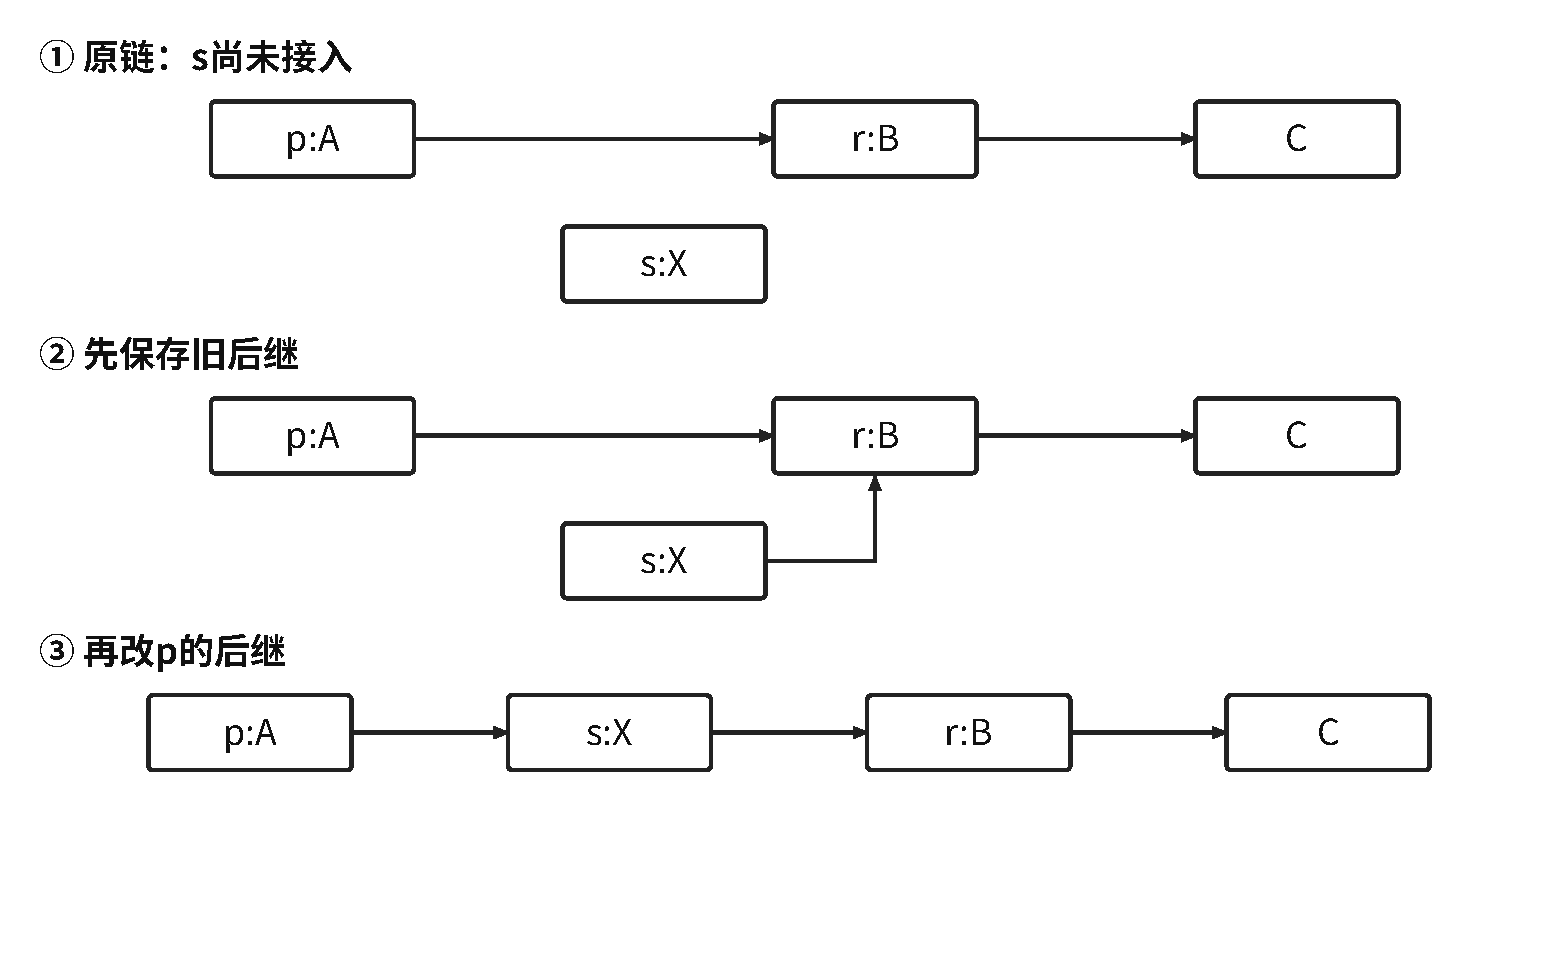
\includegraphics[width=\linewidth,height=108mm,keepaspectratio]{figures/DS_01_list_insert.pdf}
\caption{单链表后插的链接顺序}\label{DS02-insert-figure}
\end{figure}

仅给结点\(p\)，在允许改变数据与结点身份时，可通过复制数据实现前插或删自身；删除自身的复制后继法要求\(p\)有后继，尾结点不适用。共享后缀结点需统一管理释放。

不带头结点时空表为\texttt{L=\allowbreak{}=\allowbreak{}NULL}。位置1插入执行\texttt{s->\allowbreak{}next=\allowbreak{}L;\allowbreak{} L=\allowbreak{}s}；删除首元执行\texttt{p=\allowbreak{}L;\allowbreak{} L=\allowbreak{}L->\allowbreak{}next;\allowbreak{} free(\allowbreak{}p)\allowbreak{}}。修改头指针的接口须用引用或二级指针。

\subsection{建表与原地逆置}\label{DS02-build}

\par\smallskip
\begin{wideblock}
{\fontsize{9.3}{12}\selectfont\setlength{\tabcolsep}{2.5pt}\setlength{\LTleft}{0pt}\setlength{\LTright}{0pt}
\begin{longtable}{@{}>{\raggedright\arraybackslash}p{\dimexpr0.18135\linewidth-2\tabcolsep\relax}>{\raggedright\arraybackslash}p{\dimexpr0.37954\linewidth-2\tabcolsep\relax}>{\raggedright\arraybackslash}p{\dimexpr0.18135\linewidth-2\tabcolsep\relax}>{\raggedright\arraybackslash}p{\dimexpr0.25775\linewidth-2\tabcolsep\relax}@{}}
\toprule
方法 & 每轮接入 & 输入次序 & 建\(n\)结点时间 \\

\midrule\endfirsthead\toprule
方法 & 每轮接入 & 输入次序 & 建\(n\)结点时间 \\

\midrule\endhead\bottomrule\endfoot
头插 & \texttt{s-\textgreater{}next=L-\textgreater{}next;\ L-\textgreater{}next=s} & 逆序 & \(O(n)\) \\

尾插 & \texttt{r-\textgreater{}next=s;\ r=s}，结束置\texttt{r-\textgreater{}next=NULL} & 保序 & \(O(n)\)，维护尾指针 \\

\end{longtable}}
\end{wideblock}
\par\smallskip

头插前令\texttt{L->\allowbreak{}next=\allowbreak{}NULL}；尾插前令\texttt{r=\allowbreak{}L}。每轮重新寻找尾部的尾插建表需\(O(n^2)\)。教材交互式建表以9999为结束标志时，9999不能同时作为普通数据。

\par\smallskip\noindent\begin{minipage}{\linewidth}
\begin{codeblock}[language={C}]
void reverseList(LNode *L) {       // 带头结点
    LNode *prev=NULL, *cur=L->next;
    while (cur!=NULL) {
        LNode *nxt=cur->next;
        cur->next=prev;
        prev=cur;
        cur=nxt;
    }
    L->next=prev;
}
\end{codeblock}
\end{minipage}\par\smallskip

逆置维护已逆置前缀与未处理后缀，改\texttt{cur->\allowbreak{}next}前保存后继。时间\(\Theta(n)\)、辅助空间\(\Theta(1)\)，空表与单元素表均适用。

\par\medskip\Needspace{4\baselineskip}\noindent\hypertarget{DS02-E02}{}\label{DS02-E02}\textbf{例 2-2}\par\nobreak\smallskip

已知一个带有表头结点的单链表，结点结构为 \texttt{data | next}，只给出了头指针 \texttt{list}。在不改变链表的前提下，设计尽可能高效的算法，查找倒数第 \(k\) 个位置上的结点（\(k\) 为正整数）。若成功，输出该结点的 \texttt{data} 值并返回 1；否则只返回 0。要求说明设计思想、实现步骤，并用 C、C++ 或 Java 描述算法，在关键处加注释。

\section{双链表、循环链表与静态链表}\label{DS02-variants}

双链表增加\texttt{prior}域。已知有效结点后可直接取得前驱；按位查找仍需遍历。非循环链的首尾边界要检查空指针。

\par\smallskip\noindent\begin{minipage}{\linewidth}
\begin{codeblock}[language={C++}]
typedef struct DNode {
    ElemType data;
    struct DNode *prior, *next;
} DNode, *DLinklist;
bool InsertNextDNode(DNode *p, DNode *s) {
    if (p == NULL || s == NULL) return false;
    s->next = p->next;
    if (p->next != NULL) p->next->prior = s;
    s->prior = p;
    p->next = s;
    return true;
}
bool DeleteNextDNode(DNode *p) {
    if (p == NULL || p->next == NULL) return false;
    DNode *q = p->next;
    p->next = q->next;
    if (q->next != NULL) q->next->prior = p;
    free(q);
    return true;
}
\end{codeblock}
\end{minipage}\par\smallskip

\par\medskip\Needspace{4\baselineskip}\noindent\hypertarget{DS02-E03}{}\label{DS02-E03}\textbf{例 2-3}\par\nobreak\smallskip

在双链表中向 \texttt{p} 所指的结点之前插入结点 \texttt{q}，正确操作是（　）。

\par\smallskip\noindent\begin{minipage}{\linewidth}
\begin{codeblock}[language={}]
A. p->prior=q; q->next=p;
   p->prior->next=q; q->prior=p->prior;
B. q->prior=p->prior; p->prior->next=q;
   q->next=p; p->prior=q->next;
C. q->next=p; p->next=q;
   q->prior->next=q; q->next=p;
D. p->prior->next=q; q->next=p;
   q->prior=p->prior; p->prior=q;
\end{codeblock}
\end{minipage}\par\smallskip

\par\smallskip
\begin{wideblock}
{\fontsize{9.3}{12}\selectfont\setlength{\tabcolsep}{2.5pt}\setlength{\LTleft}{0pt}\setlength{\LTright}{0pt}
\begin{longtable}{@{}>{\raggedright\arraybackslash}p{\dimexpr0.32965\linewidth-2\tabcolsep\relax}>{\raggedright\arraybackslash}p{\dimexpr0.31675\linewidth-2\tabcolsep\relax}>{\raggedright\arraybackslash}p{\dimexpr0.35360\linewidth-2\tabcolsep\relax}@{}}
\toprule
表示 & 空状态 & 遍历终止或关键条件 \\

\midrule\endfirsthead\toprule
表示 & 空状态 & 遍历终止或关键条件 \\

\midrule\endhead\bottomrule\endfoot
带头普通单链表 & \texttt{L-\textgreater{}next==NULL} & 当前指针为NULL \\

带头循环单链表 & \texttt{L-\textgreater{}next==L} & 重新遇到头结点；尾满足\texttt{p-\textgreater{}next==L} \\

带头循环双链表 & \texttt{L-\textgreater{}next==L\ \&\&\ L-\textgreater{}prior==L} & 正反向均以头结点为边界 \\

无头循环单链表，仅尾指针\texttt{rear} & 空状态另行约定 & 首元为\texttt{rear-\textgreater{}next} \\

\end{longtable}}
\end{wideblock}
\par\smallskip

两个非空、无头循环单链表给定尾指针时，交换两个尾部的后继即可\(O(1)\)拼接；只给头指针通常须先找尾。带头结点版本还要删除或绕过多余头结点。

\textbf{静态链表}用数组保存结点、游标保存后继，逻辑顺序由游标决定；按逻辑位序访问仍需遍历。须管理空闲位置。例如底稿表示以0号为头结点、\texttt{next=\allowbreak{}-1}为链尾、\texttt{next=\allowbreak{}-2}为空闲，三个状态各有用途。物理地址可按数组下标寻址，不能将该下标直接作为逻辑位序。

\section{线性扫描、双指针与归并}\label{DS02-methods}

\textbf{连续删除}：指针\(p\)始终指向已处理区的最后一个保留结点；删除\(p\)后继后继续检查新后继，保留后继时才推进\(p\)。

\par\smallskip\noindent\begin{minipage}{\linewidth}
\begin{codeblock}[language={C++}]
void eraseAll(LNode* L, int x) {
    LNode* p = L;
    while (p->next != NULL) {
        if (p->next->data == x) {
            LNode* q = p->next;
            p->next = q->next;
            free(q);
        } else {
            p = p->next;
        }
    }
}
\end{codeblock}
\end{minipage}\par\smallskip

\textbf{有序数组去重}：读指针扫描，写指针维护互异前缀；仅当当前值不同于最后保留值时写入。时间\(O(n)\)、空间\(O(1)\)。无序输入仅消除相邻重复。

\textbf{有序归并}：每次输出两表当前首元素中较小者并推进对应指针，最后接余段。长度\(m,n\)的两表需\(O(m+n)\)时间。数组常需输出区；允许破坏原链表时可重接结点。稳定合并相等时先取左表；集合并集相等时只留一次并同时推进。

\par\medskip\Needspace{4\baselineskip}\noindent\hypertarget{DS02-E04}{}\label{DS02-E04}\textbf{例 2-4}\par\nobreak\smallskip

将 \(n\ (n>1)\) 个整数存放在一维数组 \(R\) 中。设计一个时间、空间都尽可能高效的算法，将序列循环左移 \(p\ (0<p<n)\) 个位置，即把 \((X_0,\ldots,X_{n-1})\) 变为 \((X_p,\ldots,X_{n-1},X_0,\ldots,X_{p-1})\)。给出思想、C/C++ 或 Java 实现，并说明时间与空间复杂度。

\par\medskip\Needspace{4\baselineskip}\noindent\hypertarget{DS02-E05}{}\label{DS02-E05}\textbf{例 2-5}\par\nobreak\smallskip

采用带头结点的单链表保存单词，两个单词可共享相同后缀的存储空间。例如 \texttt{loading} 与 \texttt{being} 共享从字符 \texttt{i} 开始的结点。\texttt{str1}、\texttt{str2} 指向两个头结点，结点为 \texttt{data | next}。设计时间上尽可能高效的算法，找到共同后缀的起始结点，给出思想、程序及时间复杂度。

\begin{figure}
\centering
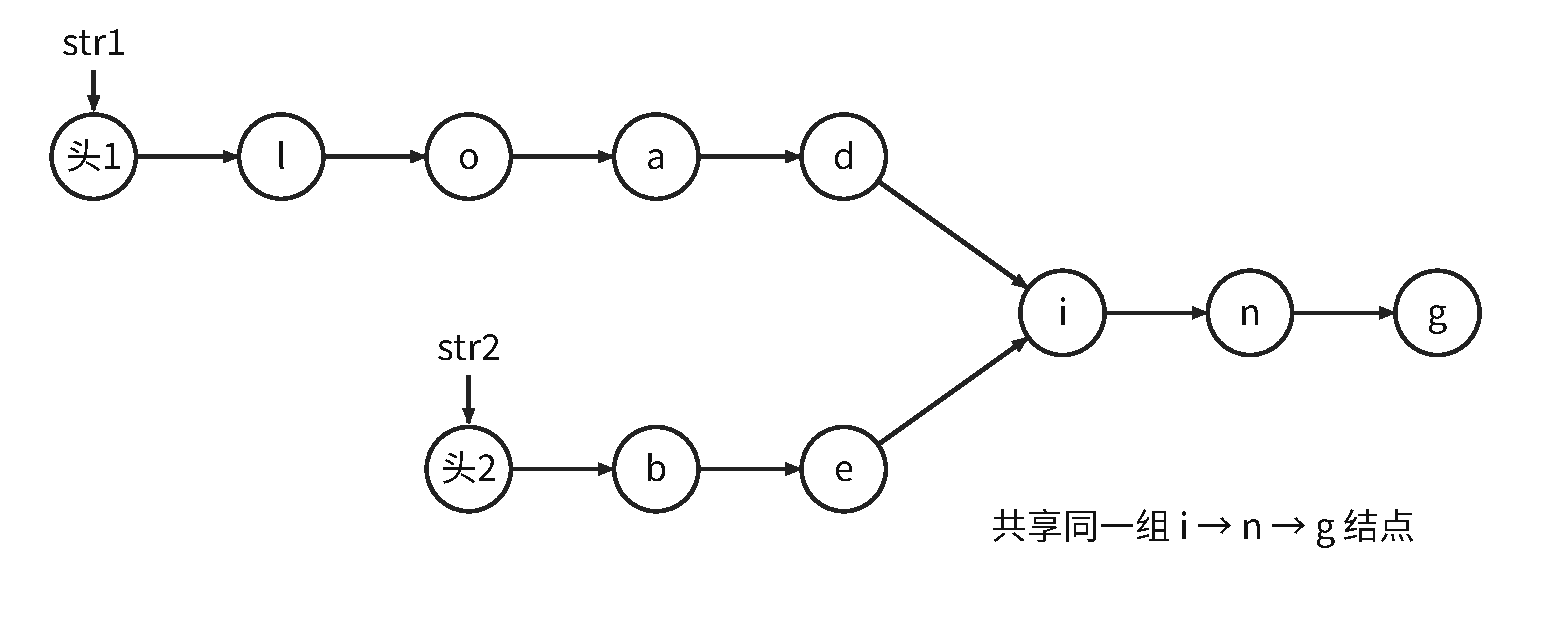
\includegraphics[width=\linewidth,height=108mm,keepaspectratio]{figures/DS_02_shared_suffix.pdf}
\caption{两个前缀分别连接到同一个 i 结点，随后共用 n、g 结点}\label{ds-fig-shared-suffix}
\end{figure}

\par\medskip\Needspace{4\baselineskip}\noindent\hypertarget{DS02-E06}{}\label{DS02-E06}\textbf{例 2-6}\par\nobreak\smallskip

整数序列 \(A=(a_0,\ldots,a_{n-1})\) 满足 \(0\le a_i<n\)。某值出现次数超过 \(n/2\) 时，称它为主元素。例如 \((0,5,5,3,5,7,5,5)\) 的主元素为5，而 \((0,5,5,3,5,1,5,7)\) 没有主元素。设计尽可能高效的算法，存在主元素时输出该值，否则输出 \ensuremath{-}1；给出思想、程序及时间、空间复杂度。

\section{顺序表与链表的操作代价}\label{DS02-comparison}

\par\smallskip
{\fontsize{9.3}{12}\selectfont\setlength{\tabcolsep}{2.5pt}\setlength{\LTleft}{0pt}\setlength{\LTright}{0pt}
\begin{longtable}{@{}>{\raggedright\arraybackslash}p{\dimexpr0.32800\linewidth-2\tabcolsep\relax}>{\raggedright\arraybackslash}p{\dimexpr0.32800\linewidth-2\tabcolsep\relax}>{\raggedright\arraybackslash}p{\dimexpr0.34401\linewidth-2\tabcolsep\relax}@{}}
\toprule
操作或资源 & 顺序表 & 带头单链表 \\

\midrule\endfirsthead\toprule
操作或资源 & 顺序表 & 带头单链表 \\

\midrule\endhead\bottomrule\endfoot
按位访问 & \(O(1)\) & \(O(n)\) \\

无序按值查找 & \(O(n)\) & \(O(n)\) \\

按位插入、删除 & 最坏\(O(n)\) & 定位最坏\(O(n)\) \\

已知前驱后插、删后继 & 仍可能搬移后缀 & \(O(1)\) \\

额外空间 & 未用容量、扩容临时区 & 每结点链接域与分配开销 \\

\end{longtable}}
\par\smallskip

顺序表连续访问具有局部性；链表适合已定位后的频繁局部修改。空间比较还要计容量利用率、链接宽度和分配开销。
